
\chapter{Numerical and Physical Accuracy}

\label{chpt:accuracy}This chapter gives a systematic comparison between
algorithms for the evaluation of $\gamma$ in terms of accuracy. The
different methods should lead to mathematical equivalent results.
The comparison for a series of CH4 with IEM and MD is done as validation
of method.


\section{Generalized spherical harmonics transform\label{sec:gsh-imp}}


\subsection{FFT}

FFT3D is implemented by package FFTW3 \citep{FFTW3} with discrete
Fourier transform (DFT) defined as: 
\begin{equation}
\begin{array}{ll}
{\displaystyle Y_{k}=\sum_{j=0}^{n-1}X_{j}e^{-2\pi ijk/n}} & \mathrm{(forward)}\end{array}
\end{equation}
\begin{equation}
\begin{array}{ll}
{\displaystyle X_{j}=\sum_{k=0}^{n-1}Y_{k}e^{2\pi ijk/n}} & \mathrm{(backward)}\end{array}
\end{equation}


Mathematically, these transforms lead to no accuracy lost. It should
be noticed that after a forward-backward Fourier transform, the original
function is multiplied by a normalization factor $N_{k}$, which is
the total number of nodes $k$. The numerical tests for selected functions
$f(x)\in\left[-5,5\right)$ (100 values) are shown in table \ref{tab:error-dft1d-1}.
\begin{table}[h]
\begin{centering}
\begin{tabular*}{1\linewidth}{@{\extracolsep{\fill}}llllc}
\toprule 
$f(x)$ & 1 & $x^{3}$ & $e^{x}$ & random number\tabularnewline
\midrule
$E_{a}^{\mathrm{max}}$ & 0 & $2.84\cdot10^{-14}$ & $3.32\cdot10^{-14}$ & \multicolumn{1}{l}{$1.80\cdot10^{-16}$}\tabularnewline
\bottomrule
\end{tabular*}
\par\end{centering}

\caption{Maximum absolute error introduced by a forward-backward (real-complex-real)
DFT1D process on a 100-value double precision array using FFTW3 package\label{tab:error-dft1d-1}}
\end{table}


We can see that the errors are about machine precision. 

The algorithmic complicity of FFT is about $\mathcal{O}(N_{k}\ln N_{k})$
\textcolor{red}{\scriptsize{}\citep{Numerical_Recipes_3ed} }, and
the computing time will be discussed in later sessions.

mmax/nmax


\subsection{$m_{\mathrm{max}}$ and $n_{\mathrm{max}}$ of projections}

The numerical error tests of a forward-backward GSHT process with
different order $m_{\mathrm{max}}$ ($m$ in table) of GSH and order
$n$ of quadrature is shown in table \ref{tab:error-gsh}.
\begin{table}[h]
\begin{centering}
\subfloat[$f(\mathbf{\Omega})=1$]{\begin{centering}
\begin{tabular*}{0.47\linewidth}{@{\extracolsep{\fill}}cccccc}
\toprule 
$m$\textbackslash{}$n$ & \multirow{1}{*}{0} & \multirow{1}{*}{1} & \multirow{1}{*}{2} & \multirow{1}{*}{3} & \multirow{1}{*}{4}\tabularnewline
\midrule
\multicolumn{1}{c}{0} &  &  &  &  & \tabularnewline
\multicolumn{1}{c}{1} &  &  &  &  & \tabularnewline
\multicolumn{1}{c}{2} &  &  &  &  & \tabularnewline
\multicolumn{1}{c}{3} &  &  &  &  & \tabularnewline
\multicolumn{1}{c}{4} &  &  &  &  & \tabularnewline
\bottomrule
\end{tabular*}
\par\end{centering}

}\subfloat[$f(\mathbf{\Omega})=\cos3\Theta$]{\begin{centering}
\begin{tabular*}{0.47\linewidth}{@{\extracolsep{\fill}}cccccc}
\toprule 
$m$\textbackslash{}$n$ & \multirow{1}{*}{0} & \multirow{1}{*}{1} & \multirow{1}{*}{2} & \multirow{1}{*}{3} & \multirow{1}{*}{4}\tabularnewline
\midrule
\multicolumn{1}{c}{0} &  &  &  &  & \tabularnewline
\multicolumn{1}{c}{1} &  &  &  &  & \tabularnewline
\multicolumn{1}{c}{2} &  &  &  &  & \tabularnewline
\multicolumn{1}{c}{3} &  &  &  &  & \tabularnewline
\multicolumn{1}{c}{4} &  &  &  &  & \tabularnewline
\bottomrule
\end{tabular*}
\par\end{centering}

}
\par\end{centering}

\begin{centering}
\subfloat[$f(\mathbf{\Omega})=\cos3\Phi$]{\begin{centering}
\begin{tabular*}{0.47\linewidth}{@{\extracolsep{\fill}}cccccc}
\toprule 
$m$\textbackslash{}$n$ & \multirow{1}{*}{0} & \multirow{1}{*}{1} & \multirow{1}{*}{2} & \multirow{1}{*}{3} & \multirow{1}{*}{4}\tabularnewline
\midrule
\multicolumn{1}{c}{0} &  &  &  &  & \tabularnewline
\multicolumn{1}{c}{1} &  &  &  &  & \tabularnewline
\multicolumn{1}{c}{2} &  &  &  &  & \tabularnewline
\multicolumn{1}{c}{3} &  &  &  &  & \tabularnewline
\multicolumn{1}{c}{4} &  &  &  &  & \tabularnewline
\bottomrule
\end{tabular*}
\par\end{centering}

}\subfloat[$f(\mathbf{\Omega})=\cos\frac{3}{2}\Psi$]{\begin{centering}
\begin{tabular*}{0.47\linewidth}{@{\extracolsep{\fill}}cccccc}
\toprule 
$m$\textbackslash{}$n$ & \multirow{1}{*}{0} & \multirow{1}{*}{1} & \multirow{1}{*}{2} & \multirow{1}{*}{3} & \multirow{1}{*}{4}\tabularnewline
\midrule
\multicolumn{1}{c}{0} &  &  &  &  & \tabularnewline
\multicolumn{1}{c}{1} &  &  &  &  & \tabularnewline
\multicolumn{1}{c}{2} &  &  &  &  & \tabularnewline
\multicolumn{1}{c}{3} &  &  &  &  & \tabularnewline
\multicolumn{1}{c}{4} &  &  &  &  & \tabularnewline
\bottomrule
\end{tabular*}
\par\end{centering}

}
\par\end{centering}

\caption{Logarithm of maximum absolute error $\lg\left(E_{a}^{\mathrm{max}}\right)$
introduced by a forward-backward GSHT process. \label{tab:error-gsh}}
\end{table}


It is shown that

It should be noticed that the tested functions are theoretically the
same if the order of quadrature / GSH is sufficient. The real case
of $\rho$ is in later session.


\subsection{From $\rho$ to $\gamma$}

Unphysical rho after transform, Gamma more smooth, Orientation 


\section{Comparison between branches}


\subsection{Error evaluation in $\hat{c}(\mathbf{k},\mathbf{\Omega_{1}},\mathbf{\Omega_{2}})$
calculation}

In appendix \ref{chpt:error-evaluation-interpolation-DCF}, we compared
the error introduced by the interpolation strategy of $\hat{c}(\mathbf{k},\mathbf{\Omega_{1}},\mathbf{\Omega_{2}})$
calculation from the intermolecular $\hat{c}(k,\boldsymbol{\omega_{1}},\boldsymbol{\omega_{2}})$.
Here, we want to compare the error introduced by \texttt{\textbf{naive\_interpolation}}
and\textbf{ }\texttt{\textbf{naive\_standard}} concerned both $\hat{c}(\mathbf{k},\mathbf{\Omega_{1}},\mathbf{\Omega_{2}})$
and the free energy and structure issued from a single-k calculation.

As shown in table , 


\subsection{A single k-kernel\label{sub:A-single-k-kernel}}

As shown in figure \ref{fig:k-kernel}, four paths are presented to
be tested, $(1)$ $(2)$ $(3)$ $(4)$

\begin{figure}[h]
\begin{centering}
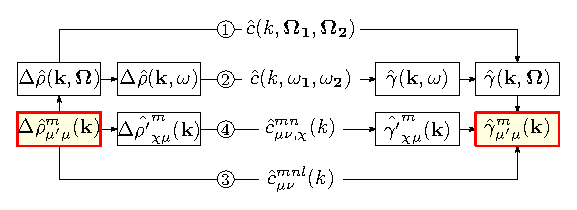
\includegraphics{_figure/algorithms_q}
\par\end{centering}

\caption{Schema of a k-kernel test \label{fig:k-kernel} }
\end{figure}


The result of error in energy for the result $\hat{\gamma}_{\mu'\mu}^{m}(\mathbf{k})$
with certain $\mathbf{k}$ is presented in table. As shown, there
is no accuracy lost for different paths in both 4 cases of $\mathbf{k}$.
This means, the final result of energy and structure is independent
to the choice of path inside a k-kernel, if $\Delta\hat{\rho}(\mathbf{k},\mathbf{\Omega})$
is a polynomial of ... as discussed in $\mathsection$\ref{sec:gsh-imp}.

\begin{table}[h]
\begin{centering}
\begin{tabular*}{1\linewidth}{@{\extracolsep{\fill}}llll}
\toprule 
$\mathbf{k}$ & $E_{2}^{\max}$ & $E_{3}^{\max}$ & $E_{4}^{\max}$\tabularnewline
\midrule
$(2,3,5)$ &  &  & \tabularnewline
$(4,0,1)$ &  &  & \tabularnewline
$(0,0,0)$ &  &  & \tabularnewline
$(0,0,1)$ &  &  & \tabularnewline
\bottomrule
\end{tabular*}
\par\end{centering}

\caption[Maximum absolute error introduced by paths of a k-kernel test]{Maximum absolute error introduced by paths $(1)\ldots(4)$ shown
figure \ref{fig:k-kernel}, using an input $\Delta\hat{\rho}_{\mu'\mu}^{m}(\mathbf{k})$
issue of MDFT minimization. $\mathbf{k}$ is of unity $[\mathrm{\textrm{\AA}^{-3}}]$.
For special case $\mathbf{k}=(0,0,0)$, ... $E_{i}^{\max}$ is the
absolute difference between path (1) and path ($i$).\label{tab:error-k-kernel}}
\end{table}



\subsection{k-border effect\label{sub:k-border-effect}}

\begin{table}[h]
\begin{centering}
\begin{tabular*}{1\linewidth}{@{\extracolsep{\fill}}llll}
\toprule 
 & \texttt{\textbf{convolution\_standard}} & \texttt{\textbf{convolution\_asymm}} & \texttt{\textbf{convolution\_pure\_angular}}\tabularnewline
\midrule
$E_{\gamma}^{\max}$(64) &  &  & \tabularnewline
$\mathcal{F}_{\mathrm{exc}}$ (64) &  &  & \tabularnewline
$E_{\gamma}^{\max}$(65) &  &  & \tabularnewline
$\mathcal{F}_{\mathrm{exc}}$ (65) &  &  & \tabularnewline
\bottomrule
\end{tabular*}
\par\end{centering}

\caption[Error in $\gamma(\mathbf{r},\mathbf{\Omega})$ and $\mathcal{F}_{\mathrm{exc}}$
before border correction]{Maximum absolute error introduced by different branches in calculated
$\gamma(\mathbf{r},\mathbf{\Omega})$ and the difference in $\mathcal{F}_{\mathrm{exc}}$
from a given $\Delta\rho_{\mu'\mu}^{m}(\mathbf{r})$ compared to \texttt{\textbf{naive\_standard}}
before border correction for a $64^{3}$ and $65^{3}$ spatial grid,
$n_{\max}=5$.}
\end{table}


standard, asymm and pure\_angular different because...

In MDFT, the symmetry 
\begin{equation}
\Delta\hat{\rho'}_{\chi\mu}^{m}(\mathbf{k})=(-)^{m+\mu+\chi}\Delta\hat{\rho'}_{\chi,-\mu}^{m*}(-\mathbf{k})\label{eq:2-1}
\end{equation}
 is generated by two symmetries

\begin{equation}
\Delta\hat{\rho}_{\mu'\mu}^{m}(\mathbf{k})=(-)^{\mu'+\mu}\Delta\hat{\rho}_{-\mu',-\mu}^{m*}(-\mathbf{k})\label{eq:1-1}
\end{equation}


\begin{equation}
R_{\mu'\chi}^{m}(\hat{k})=(-)^{m+\mu'+\chi}R_{-\mu',\chi}^{m}(-\hat{k})\label{eq:3-1}
\end{equation}


For the points ``at border'', it's to say that after the FFT where
the point having $\pm k_{i}=k_{i}^{\mathrm{max}}$, $i=1,2,3$, for
example for $k_{1},$

\[
\Delta\hat{\rho}_{\mu'\mu}^{m}(\pm k_{1},k_{2},k_{3})=\Delta\hat{\rho}_{\mu'\mu}^{m}(k_{1}^{\mathrm{max}},k_{2},k_{3})
\]
is naturally put in the same array by FFT for the grids having even
number. \marginpar{For example, for a grid 1D, the FFT having 6 points gives the values
for indices 0,1,2,3,-2,-1, and the FFT having 7 points gives the values
for 0,1,2,3,-3,-2,-1.}

But

\[
R_{-\mu',\chi}^{m}(-\hat{k}\equiv(-k_{1},-k_{2},-k_{3}))\neq R_{\mu',\chi}^{m}(k_{1}^{\mathrm{max}},-k_{2},-k_{3})
\]
Thus the symmetries (\ref{eq:3-1}) and (\ref{eq:2-1}) are not respected
for these points 

In the backward process, if we make sense of all the $\gamma_{\mu'\mu}^{m}(\mathbf{k})$,
as

\[
\gamma_{\mu'\mu}^{m}(-\hat{k}\equiv(-k_{1},-k_{2},-k_{3}))\neq\gamma_{\mu'\mu}^{m}(k_{1}^{\mathrm{max}},-k_{2},-k_{3})
\]
the symmetry

\begin{equation}
\gamma_{\mu'\mu}^{m}(\mathbf{k})=(-)^{\mu'+\mu}\gamma_{-\mu',-\mu}^{m*}(-\mathbf{k})\label{eq:1-1}
\end{equation}
is not respected totally, and this imposes that $\gamma_{\mu'\mu}^{m}(\mathbf{r})$
have a imaginary part. In the version FFTW3, we keep only the part
of none-negative $\mathbf{k}$ or none-negative, supposing that the
part we omit respects the symmetry.

\begin{figure}[h]
\begin{centering}
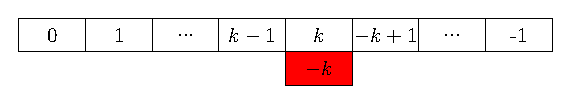
\includegraphics{_figure/k-border}
\par\end{centering}

\caption{k-border effet}
\end{figure}


\begin{table}[h]
\begin{centering}
\begin{tabular*}{1\linewidth}{@{\extracolsep{\fill}}llll}
\toprule 
 & \texttt{\textbf{convolution\_standard}} & \texttt{\textbf{convolution\_asymm}} & \texttt{\textbf{convolution\_pure\_angular}}\tabularnewline
\midrule
$E_{\gamma}^{\max}$(65) &  &  & \tabularnewline
$\mathcal{F}_{\mathrm{exc}}$ (65) &  &  & \tabularnewline
\bottomrule
\end{tabular*}
\par\end{centering}

\caption[]{Maximum absolute error introduced by different branches after border
correction}
\end{table}


\begin{figure}
\caption{structure of gamma in rotational invariants}
\end{figure}


the mysterious error between \texttt{\textbf{naive\_standard}} and
the \texttt{\textbf{convolution}} branches cannot explained, this
implied that there is probably a bug in \texttt{\textbf{naive\_standard}}. 


\section{Intrinsic variation of free energy}

Before study of free energy dependence on angular algorithms, we are
interested in the grid dependance, with can have an influence in the
follow tests.


\subsection{Spatial grid: length and resolution}


\subsection{Angular grid: effect of psi}


\section{Series of charged LJ centre}

charged $\mathrm{C}\mathrm{H}_{4}$ centre

\begin{table}
\begin{centering}
\begin{tabular*}{1\linewidth}{@{\extracolsep{\fill}}llllllll}
\toprule 
charge  & sigma {[}{]} & epsilon {[}{]} & x {[}$\textrm{\AA}${]} & y {[}$\textrm{\AA}${]} & z {[}$\textrm{\AA}${]} & temperature {[}K{]} & number density of solvent\tabularnewline
\midrule
-1.0 to 1.0 & 3.73  & 1.23  & 0 & 0 & 0 & 298 & 0.0332891\tabularnewline
\bottomrule
\end{tabular*}
\par\end{centering}

\caption{Parameters of charged Lenard-Jones centre (modified from $\mathrm{C}\mathrm{H}_{4}$) }
\end{table}


here we use 298K according to habitude instead of 303K recommended
in reference \textcolor{red}{{[}ref{]}}.


\subsection{Box length dependance and charge dependance of free energy}

As discussed in section \ref{chpt:thermodynamic-quantities}, for
single ions, two types of corrections need to be added on the free
energy, which depend on the box length and and charge of the ion.
To verify these dependence, we implement a systematic calculation
from charge shown in figure

\begin{figure}
\caption{free energy (without correction) of charged $\mathrm{C}\mathrm{H}_{4}$
centre (-1.0 to 1.0) with respect to the box length}
\end{figure}


Continuum model correction at boundary

\begin{figure}
\caption{Parabolic charge dependence of free energy of $\mathrm{C}\mathrm{H}_{4}$
centre series}
\end{figure}


It satisfies the Born model.

memory leak can cause divergence.


\subsection{Comparison with IET}

\begin{figure}
\caption{Linear dependence of charge in the comparison to IET. Old algorithm
/ new algorithm, without correction}
\end{figure}


\begin{figure}
\caption{Comparison to IET. Old algorithm / new algorithm, with P-scheme correction}
\end{figure}


Old data in appendix \ref{chpt:original_data}, which use 2m phi.
It gives quite similar result, which shows the insensibility of grid.


\subsection{Comparison with DM }


\section{Premier conclusion}

Capable to produce the same result with IEM, but have more ability
to calculate 3D molecules which is not suitable for spherical coordinates.
